\documentclass[11pt]{article}
\usepackage[T1]{fontenc}
\usepackage{amsmath,amssymb,graphicx}
\usepackage[margin=1in]{geometry}
\usepackage{hyperref}
\hypersetup{hidelinks}
\setlength{\emergencystretch}{3em}
\setlength{\parskip}{4pt}
\newcommand{\dd}{\mathrm d}
\newcommand{\Ds}{D_s}
\newcommand{\I}{\mathcal I}
\newcommand{\U}{U_{\mathrm{int}}}
\newtheorem{postulate}{Postulate}
\newtheorem{proposition}{Proposition}
\title{Foundations of a Geometric Identity Theory:\\Worldline Structure, Layered State, and Coupled Dynamics}
\author{Jason D. Dutton\\Castlewood, Virginia, USA}
\date{October 17, 2026\\\small Foundational author-review draft}
\begin{document}
\maketitle
\begin{abstract}
We propose a geometric identity framework in which a history carries both a spacetime worldline and an internal layered state. The motivating hypothesis is that continuity of entity identity can be studied through geometry, while changes of expression are represented by internal evolution. Four internal coordinates, labeled Origin, Authorship, Sovereignty, and Warp, are introduced independently of a scalar identity observable. A minimal classical realization couples these coordinates to proper curvature and first torsion through one stationary action. The internal equations, a separately conserved Origin energy, and the higher-derivative geometric variational equation are stated on a regular timelike domain. For prescribed constant geometry, stationary internal configurations and a positive-Hessian condition for local Lyapunov stability are obtained. An exact oscillator example distinguishes bounded evolution from attraction, while square completion identifies a limitation of geometric control by the proposed potential. The single-entity interpretation, quantum field emergence, and possible spectral or computational extensions are presented as research hypotheses rather than consequences of the classical construction. The resulting document establishes a common vocabulary, an explicit mathematical starting point, and a sequence of tests required to assess the theory.
\end{abstract}

\section{The foundational question}
What mathematical structure can represent an entity that remains identifiable while its geometric history and local expression change? This proposal treats that question as a joint problem of geometry, internal state, and dynamics. A history is described by a spacetime curve together with a layered identity state, and a common action specifies their interaction. The aim is to make continuity, transformation, and stability precise enough to analyze rather than infer their properties from names.

The motivating physical interpretation is that a continuous geometric entity may underlie multiple observed manifestations. That interpretation is a hypothesis about ontology. The classical model developed here studies one regular history and its internal variables; it does not demonstrate that one smooth curve represents all particles, all admissible paths, or an electron quantum field. The mathematical distinction between a particular history and an ensemble of histories remains essential.

Established worldline methods provide a useful context: some quantum-field-theoretic quantities admit particle path-integral representations.\cite{strassler,schubert} Such representations do not independently establish a single-entity ontology. The present program asks whether an additional identity structure can be formulated consistently and connected to observables. It begins with a classical realization so that assumptions and consequences can be separated before quantization is attempted.

The framework has three roles, introduced together here. Worldline geometry describes where and how a history is embedded. Layered identity describes its internal state. Coupled dynamics specifies how the two influence one another. The labels GWFM, SEFI, and DEFI have been used in the author's working manuscripts for these roles;\cite{gwfm,sefi,defi,sefispace,unified} none is treated as an independently established physical theory on which the reader must rely. This document is self-contained in its postulates and classical equations. The previous manuscripts are cited for provenance.

\begin{figure}[htbp]
\centering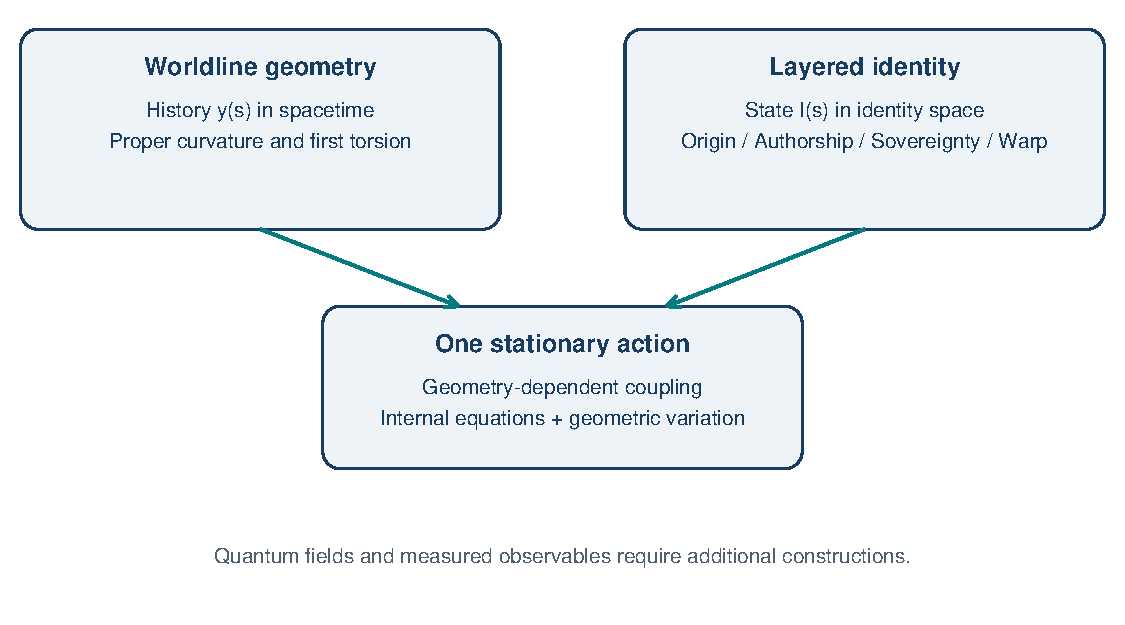
\includegraphics[width=\linewidth]{figures/01-architecture.pdf}
\caption{The proposed classical architecture. Geometry and internal state enter one action and are varied jointly. The arrows indicate dependence in the variational model, not measured causal channels. A bridge to quantum fields or detector outcomes is a separate task.}\label{fig:architecture}
\end{figure}

\section{Conceptual vocabulary and scope}
\subsection{Entity, history, and manifestation}
An entity is the proposed persisting object of description. A classical history is a map $z=(y,I)$ into spacetime times identity space. A manifestation would be an observable attributed to that history under specified measurement conditions. The first two notions can be represented by the variables below. The third requires an observation law; it is not supplied by assigning a layer name or taking a scalar sum.

In particular, a continuous map from an interval, a set of allowed maps, a probability law on maps, and a quantum amplitude over maps are different objects. The foundational single-entity hypothesis does not identify them by definition. To connect them, the theory must specify how histories are selected, weighted, and related to observations.

\subsection{Four layers as modeling roles}
\begin{description}
\item[Origin] Records the foundational internal sector. In the minimal realization it is an autonomous oscillator whose energy is conserved; its coordinate need not be constant.
\item[Authorship] Modulates the coupling of internal state to geometric invariants. This is a constitutive choice, not an assertion of intention or agency in a physical field.
\item[Sovereignty] Names the persistence and invariance problem. Its coordinate enters a curvature coupling, while actual invariance requires a separately stated transformation and preserved quantity.
\item[Warp] Names permitted transformation of expression. Its coordinate enters a first-torsion coupling in the example studied here. Neither this use of the word nor the action supplies a spacetime propulsion mechanism.
\end{description}
These labels guide interpretation while the equations determine the mathematical content. They are not measured particle properties, symmetry generators, or quantum numbers without further definitions. No fifth dynamical coordinate is assumed. A Reality or manifestation layer used in an earlier overview\cite{overview} is left as an observational question rather than silently promoted to another oscillator.

\subsection{Postulates of the minimal realization}
\begin{postulate}[Geometric history]
A classical history contains a smooth timelike immersed curve in time-oriented Minkowski spacetime. The torsion-coupled realization is restricted to nonzero proper curvature on the interval considered.
\end{postulate}
\begin{postulate}[Independent layered state]
Each history carries four independent real internal coordinates on a fixed affine identity space. A positive constant metric specifies internal kinetic weights. A scalar identity observable is an additional chosen contraction, not a replacement for the full state.
\end{postulate}
\begin{postulate}[Common dynamics]
Geometry and identity enter one reparametrization-invariant action. The action below is the minimal constitutive example studied in this document; its coupling functions and positive stiffnesses are model inputs.
\end{postulate}
\begin{postulate}[Explicit invariance]
Any claim of sovereignty identifies what is preserved and under which transformations. A symmetry of observables, a symmetry of the action, a conserved quantity, and a flow-invariant set are distinct mathematical requirements.
\end{postulate}
The postulates specify a candidate model, not empirical laws. Its empirical interpretation requires a map to observations, parameter identification, and comparison with existing theory.

\section{Mathematical setting and notation}
We use $c=\hbar=1$. Greek indices label spacetime components and $a$ ranges over $O,A,S,W$. The arbitrary curve parameter is $\lambda$ and proper time is $s$; $\Ds$ means $\dd/\dd s$. Curvature is $\kappa$ and first torsion magnitude is $\tau_1$, never a time parameter. $H$ denotes the internal kinetic metric, $k_a$ the stiffnesses, $F$ a scalar identity observable, and $\U$ the internal--geometric coupling. The action is $S[y,I]$; the symbol $I_S$ denotes the Sovereignty coordinate, not the action. A prime on a coupling function differentiates its scalar argument.
\subsection{Timelike geometry and its domain}
We work in flat Minkowski spacetime $M=\mathbb R^{1,3}$ with signature $(-,+,+,+)$ and $c=\hbar=1$. Curved-spacetime extensions require additional connection and boundary analysis and are not proved here. Let $y(\lambda)$ be a smooth timelike immersion on a finite interval and define
\begin{equation}
 v=\sqrt{-\eta_{\mu\nu}y'^{\mu}y'^{\nu}}>0,
 \qquad \dd s=v\dd\lambda,\qquad
 \Ds=v^{-1}\dd/\dd\lambda .
 \label{eq:proper}
\end{equation}
A prime on $y$ means $\lambda$ differentiation. Set $T=\Ds y$, $a=\Ds T$, and $\kappa=\sqrt{\eta(a,a)}$. On the domain $\kappa>0$, define
\begin{equation}
 N=a/\kappa,\qquad b=\Ds N-\kappa T,
 \qquad \tau_1^2=\eta(b,b).
 \label{eq:frenet}
\end{equation}
Differentiating $\eta(T,N)=0$ gives $\eta(T,\Ds N)=-\kappa$; thus $b$ is orthogonal to both $T$ and $N$. It lies in a positive definite normal plane and $\tau_1^2\geq0$. Where $\tau_1>0$, $B=b/\tau_1$ yields $\Ds N=\kappa T+\tau_1B$. Four-dimensional curves can have another Frenet invariant, which this ansatz does not use. The square $\tau_1^2$ remains defined at $b=0$ when $\kappa>0$, even though $B$ is then undefined.

Curvature depends on second derivatives of $y$ and first torsion generally on third derivatives. At $\kappa=0$, Eq.~\eqref{eq:frenet} is undefined. We do not assign torsion to a straight worldline by fiat. A straight-curve limit requires a separate smooth extension of the torsion term or removal of that term. Admissible local variations stay within $v>0$ and $\kappa>0$; existence through the singular boundary is an open problem.

The proper curvature is the magnitude of proper acceleration. A coordinate-time acceleration bound is a different statement and depends on the chosen frame. No universal upper bound on either quantity is imposed or derived by the present action.

\subsection{Independent identity coordinates and scalar observables}
The minimal internal space is a fixed affine space $\I=\mathbb R^4$, with labels
\begin{equation}
I=(I_O,I_A,I_S,I_W),\qquad F=\ell_a I^a,\qquad\ell=(1,1,1,1).\label{eq:identity}
\end{equation}
The coordinates are dimensionless real variables; labels on their subscripts do not denote metric lowering. They do not transform as a spacetime four-vector. We prescribe the constant positive kinetic metric $H=\operatorname{diag}(h_O,h_A,h_S,h_W)$ and a separate positive stiffness matrix. These are model data.

The vector and its scalar contraction have distinct roles. $I$ specifies the internal configuration; $F$ is one chosen observable. Since $\ell$ has a three-dimensional kernel, $F$ does not determine $I$. In particular, $I$ and $I+(u,-u,0,0)$ have the same sum. Independent internal dynamics are therefore an additional postulate, not a consequence of adding four scalar layer functions. The covector $\ell$ must transform along with coordinates if the same observable is described in another internal basis. Figure~\ref{fig:scalar} makes this distinction explicit.
\begin{figure}[htbp]
\centering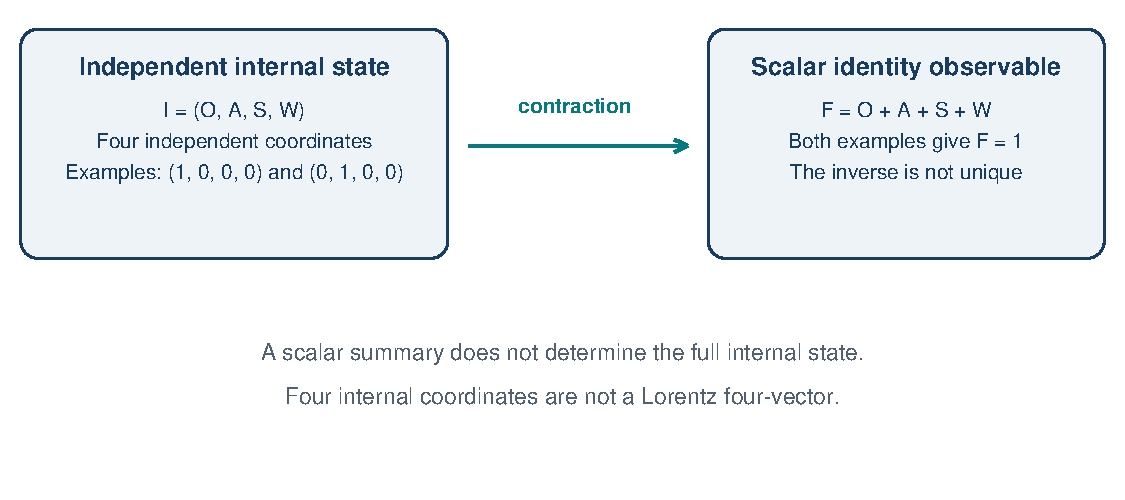
\includegraphics[width=\linewidth]{figures/02-scalar-vector.pdf}
\caption{The identity vector contains more information than a scalar identity observable. The two states shown are examples of equal scalar contraction, not equivalent physical states established by the theory.}\label{fig:scalar}
\end{figure}

The four layer names identify modeling roles. They do not supply a gauge group, a conserved charge, or measured observables by themselves. An allowed transformation class must be specified before requiring scalar invariance $F(g\cdot z)=F(z)$ or vector invariance. Invariance of $F$ under a transformation is different from constancy of $F$ along evolution.

\subsection{Parameters and units}
We use positive stiffnesses $k_a$ and oscillator frequencies $\omega_a^2=k_a/h_a$, with dimensionless $I^a$. In natural units $[s]=L$, $[m]=L^{-1}$, $[h_a]=L$, $[k_a]=L^{-1}$, $[\kappa]=[\tau_1]=L^{-1}$, and the coupling functions $\mu_j$ have dimension $L$. A convention identifying numerical inertial and stiffness coefficients is available only after choosing dimensionless time and corresponding scales. Couplings are at least $C^2$ for the Hessian analysis and smooth where higher geometric derivatives are used.

\section{A minimal coupled action}
The joint configuration space is $M\times\I$, but the geometry-dependent Lagrangian is defined on its higher jet space. The proposed action is
\begin{align}
 S[y,I]&=\int\dd s\left[-m+\tfrac12\sum_a h_a(\Ds I^a)^2-V(I;\kappa,\tau_1)\right],\label{eq:action}\\
 V&=\tfrac12\sum_a k_a(I^a)^2+\U,\label{eq:potential}\\
 \U&=\mu_1(I_A)\kappa^2 I_S+\mu_2(I_A)\tau_1^2 I_W.\label{eq:coupling}
\end{align}
In a general parameter, $S=\int\mathcal L\dd\lambda$ with $\mathcal L=v[-m+\frac12\sum h_a(I'^a/v)^2-V]$. This makes the dependence of the proper-time measure on the varied curve explicit. Orientation-preserving reparametrizations leave the action unchanged. Fixing $v=1$ before varying $y$ without imposing its constraint would lose terms and is not legitimate.

The coupling is phenomenological. It associates sovereignty with curvature, warp with torsion, and authorship with coupling strength, as a declared constitutive choice. These associations are not unique; a geometric transformation may change both invariants. Origin is absent from $\U$ by a separate decoupling assumption. Joint variation gives reciprocal influence, but there is no exchange symmetry between the inequivalent geometry and identity sectors.

\subsection{Internal Euler--Lagrange equations}
Holding $y$ fixed and varying $I$ with vanishing endpoint variations gives
\begin{align}
 h_O\Ds^2 I_O+k_O I_O&=0,\label{eq:origin}\\
 h_S\Ds^2 I_S+k_S I_S+\mu_1(I_A)\kappa^2&=0,\label{eq:S}\\
 h_W\Ds^2 I_W+k_W I_W+\mu_2(I_A)\tau_1^2&=0,\label{eq:W}\\
 h_A\Ds^2 I_A+k_A I_A
 +\mu_1'(I_A)\kappa^2 I_S+\mu_2'(I_A)\tau_1^2 I_W&=0.\label{eq:A}
\end{align}
Here a prime on $\mu_j$ differentiates its scalar argument. Together with the geometric variational equation, these equations specify the proposed classical coupling. Their derivation uses fixed geometry only during the internal variation, not as a restriction on all joint stationary histories.

\subsection{Geometric variation and boundary data}
Since $\mathcal L$ generally depends on $y',y'',y'''$, its coordinate Euler--Lagrange equation in Minkowski space is
\begin{equation}
 \frac{\partial\mathcal L}{\partial y^\mu}
 -\frac{\dd}{\dd\lambda}\frac{\partial\mathcal L}{\partial y'^\mu}
 +\frac{\dd^2}{\dd\lambda^2}\frac{\partial\mathcal L}{\partial y''^\mu}
 -\frac{\dd^3}{\dd\lambda^3}\frac{\partial\mathcal L}{\partial y'''^\mu}=0.
 \label{eq:EL}
\end{equation}
For this translation-invariant ansatz the first term vanishes. Equation~\eqref{eq:EL}, with $\mathcal L$ as defined above, is a variational characterization rather than an expanded sixth-order initial-value system. We fix $y,y',y''$ at the endpoints, or use compactly supported variations. Other boundary choices require natural boundary conditions. Reparametrization invariance produces a differential identity between the equations, so constraint analysis is needed before counting independent degrees of freedom.

One can see the feedback without assuming a solution. In proper-time notation the coupling contribution to a geometric first variation includes
\begin{equation}
 \delta_y S_{\rm coupling}
 =-\int\dd s\left[2\mu_1 I_S\kappa\,\delta_y\kappa
       +\mu_2 I_W\delta_y(\tau_1^2)\right]
   -\int \U\,\delta_y(\dd s).
 \label{eq:feedback}
\end{equation}
The rest of the action has measure and kinetic variations as well. Vanishing internal acceleration does not remove Eq.~\eqref{eq:feedback}. The curvature and torsion terms originate in the declared coupling; they are not implicit terms in the length action.

Higher derivatives raise a separate Hamiltonian question. Nondegenerate higher-derivative systems fall under the Ostrogradsky instability mechanism.\cite{woodard} This action has gauge degeneracies, so that theorem cannot be applied without examining the constrained highest-derivative Hessian. We establish neither ghost freedom nor inevitable instability of every solution. A complete reduced Hamiltonian and local well-posedness analysis remain necessary.

\section{Conservation, balance, and conditional stability}
\subsection{A separately conserved Origin energy}
\begin{proposition}
Along every smooth solution of Eq.~\eqref{eq:origin},
\begin{equation}
 Q_O=\tfrac12 h_O(\Ds I_O)^2+\tfrac12 k_O I_O^2
 \label{eq:Q}
\end{equation}
is constant in proper time.
\end{proposition}
\textit{Proof.} Direct differentiation gives
\begin{equation}
 \Ds Q_O=(\Ds I_O)(h_O\Ds^2 I_O+k_O I_O)=0.
\end{equation}
This uses the absence of Origin couplings and constant $h_O,k_O$, not an assertion that $I_O$ itself is constant. For the autonomous Origin oscillator on prescribed geometry, $Q_O$ is its time-translation Noether energy.\cite{noether} In the coupled reparametrization-invariant problem the direct first integral is sufficient; we do not identify it with an electromagnetic charge or a total spacetime energy.

For prescribed geometry the full internal energy obeys
\begin{align}
 E_I&=\tfrac12\sum_a h_a(\Ds I^a)^2+V,\\
 \Ds E_I&=2\mu_1 I_S\kappa\Ds\kappa
             +\mu_2 I_W\Ds(\tau_1^2).
 \label{eq:energy}
\end{align}
The internal system can exchange energy with varying geometry. If both geometric invariants are constant, $E_I$ is conserved. This fact does not amount to conservation of $E_I$ along arbitrary coupled solutions.

\subsection{Prescribed constant geometry}
Let $\kappa=\bar\kappa>0$ and $\tau_1=\bar\tau$ be prescribed constants. An internal equilibrium has both $\Ds I=0$ and $\nabla_I V=0$. Its Origin coordinate is zero, and its other coordinates satisfy
\begin{align}
 I_S^*&=-\mu_1(A_*)\bar\kappa^2/k_S,\label{eq:IstarS}\\
 I_W^*&=-\mu_2(A_*)\bar\tau^2/k_W,\label{eq:IstarW}\\
 0&=k_A A_*-
 \mu_1'(A_*)\mu_1(A_*)\bar\kappa^4/k_S
 -\mu_2'(A_*)\mu_2(A_*)\bar\tau^4/k_W.\label{eq:Astar}
\end{align}
There may be no root, one root, or several. The algebraic balance set for varying geometry is located in jet space, where $\kappa$ and $\tau_1$ are defined, rather than merely in $M\times\I$. We reserve ``equilibrium'' for a state whose full internal phase-space velocity vanishes.

\begin{proposition}[Conditional internal stability]
At a root $A_*$ of Eq.~\eqref{eq:Astar}, the internal potential Hessian is positive definite if and only if
\begin{equation}
 \Delta=k_A-
 \frac{(\mu_1'^2+\mu_1\mu_1'')\bar\kappa^4}{k_S}
 -\frac{(\mu_2'^2+\mu_2\mu_2'')\bar\tau^4}{k_W}>0,
 \label{eq:schur}
\end{equation}
where the coupling functions and derivatives are evaluated at $A_*$. Under this condition the equilibrium is locally Lyapunov stable in the internal system with prescribed constant geometry. It is not asymptotically attracting.
\end{proposition}
\textit{Proof.} Origin contributes a positive one-dimensional block $k_O$. In the ordered coordinates $(A,S,W)$ the remaining Hessian is
\begin{equation}
 K=\begin{pmatrix}
 k_A+\mu_1''\bar\kappa^2I_S^*+\mu_2''\bar\tau^2I_W^*&\mu_1'\bar\kappa^2&\mu_2'\bar\tau^2\\
 \mu_1'\bar\kappa^2&k_S&0\\
 \mu_2'\bar\tau^2&0&k_W
 \end{pmatrix}.
\end{equation}
The Schur complement of the positive diagonal $(k_S,k_W)$ block is Eq.~\eqref{eq:schur}. Positive definiteness gives a strict local minimum of $V$. Conservation of the positive kinetic energy plus the potential difference confines sufficiently small initial perturbations to a neighborhood of that minimum. Linearization yields $H\Ds^2\xi+K\xi=0$ with positive squared frequencies. Conservation also precludes convergence from all nearby higher-energy states. $\square$

This result concerns internal variables on fixed geometry. If $\Delta<0$, the Hessian has a negative direction and the internal linearized system has an exponentially growing mode. If $\Delta=0$, nonlinear terms must be examined. For varying geometry, instantaneous positive Hessians alone do not preclude parametric excitation.

\subsection{An exact bounded example and a global obstruction}
For constant $\mu_1=c_1$ and $\mu_2=c_2$, the internal equilibrium is unique: $A_*=I_O^*=0$ and Eqs.~\eqref{eq:IstarS}--\eqref{eq:IstarW} fix the other coordinates. For example,
\begin{equation}
 I_S(s)=I_S^*+C_S\cos(\omega_Ss)+D_S\sin(\omega_Ss).
 \label{eq:forced}
\end{equation}
There are analogous solutions for $I_W,I_A,I_O$. The deviations remain bounded and generically oscillate forever. Boundedness is not relaxation, and does not constrain the worldline's proper acceleration. Figure~\ref{fig:oscillator} shows the exact internal behavior.
\begin{figure}[htbp]
\centering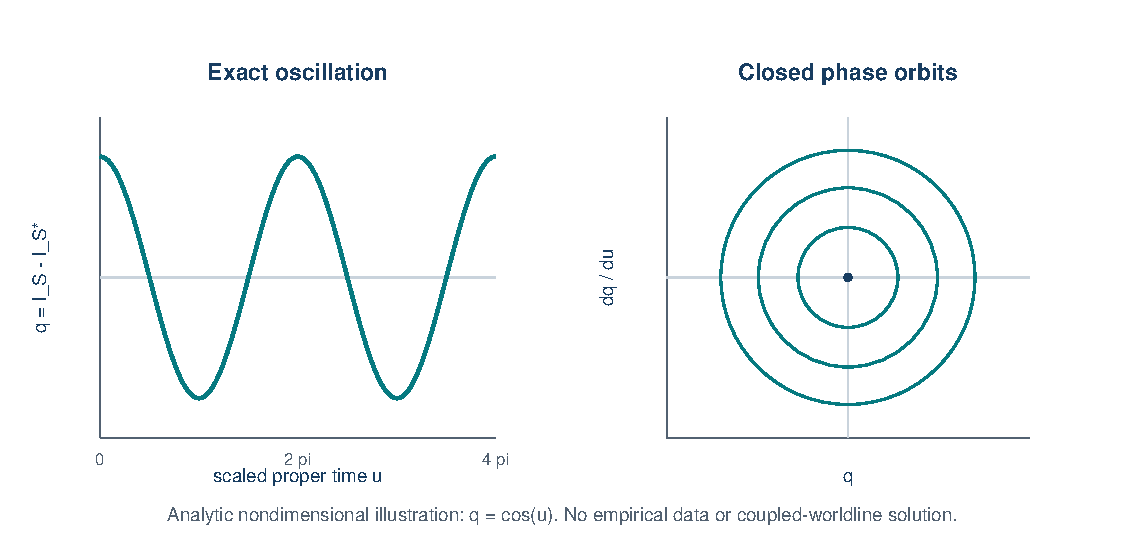
\includegraphics[width=\linewidth]{figures/03-exact-dynamics.pdf}
\caption{Exact internal motion for constant prescribed geometry and constant coupling. With $u=\omega_Ss$ and unit deviation amplitude, $q=I_S-I_S^*=\cos u$. Phase curves are circles in $(q,\dd q/\dd u)$ coordinates. Closed orbits illustrate bounded conservative motion, not relaxation. This is an analytic illustration, not experimental data or a solution of the full coupled geometric equations.}\label{fig:oscillator}
\end{figure}


Completing squares in the general potential gives
\begin{align}
 V={}&\tfrac12 k_O I_O^2+\tfrac12 k_A I_A^2
 +\tfrac12 k_S\left(I_S+\frac{\mu_1\kappa^2}{k_S}\right)^2\nonumber\\
 &+\tfrac12 k_W\left(I_W+\frac{\mu_2\tau_1^2}{k_W}\right)^2
 -\frac{\mu_1^2\kappa^4}{2k_S}
 -\frac{\mu_2^2\tau_1^4}{2k_W}.
 \label{eq:negative}
\end{align}
At fixed $I_A$ with a nonzero coupling, allowing its associated geometric invariant to grow lowers this internal effective potential without bound. This algebraic observation does not by itself prove that the constrained full Hamiltonian is unbounded, since geometric invariants are derivative variables. It does show that internal oscillator positivity supplies no coercive control of geometry. Adding stabilizing terms, restricting admissible invariants, or using an effective-theory cutoff would alter the model and needs an independent justification.

\subsection{Why acceleration-zero balance is not invariance}
A possible ideal-evolution condition can be stated on $\I=\mathbb R^4$:
\begin{equation}
 \Ds(\kappa,\tau_1,\Ds I,\Ds^2I)
 =(\Ds\kappa,\Ds\tau_1,\Ds^2I,\Ds^3I)=0.
 \label{eq:invariant}
\end{equation}
The entries have different units and form a tuple, not a single vector with an unspecified common covariant derivative. A genuine invariant locus must be preserved by the full phase-space flow. Solving Eqs.~\eqref{eq:IstarS}--\eqref{eq:Astar} at one instant proves neither $\Ds\kappa=\Ds\tau_1=0$ nor $\Ds^3I=0$.

For an explicit counterexample, take constant prescribed geometry and constant couplings; leave $I_A,I_S,I_W$ at equilibrium and choose
\begin{equation}
 I_O(s)=\epsilon\sin(\omega_Os),\qquad \epsilon\ne0.
\end{equation}
At $s=0$ every internal acceleration vanishes, but
\begin{equation}
 \Ds I_O(0)=\epsilon\omega_O\ne0,\qquad
 \Ds^3I_O(0)=-\epsilon\omega_O^3\ne0.
\end{equation}
Thus acceleration-zero balance does not imply Eq.~\eqref{eq:invariant}, even before geometric feedback is considered. Setting $\Ds I=0$ and $I=I^*$ with constant prescribed invariants does give an internal stationary solution. Realizing it as a full solution also requires Eq.~\eqref{eq:EL} and its constraints. No such general full-system existence or attracting-manifold theorem is claimed.


\section{From a classical history to physical fields}
\subsection{A defined occupation distribution}
A limited field-like construction is available without quantization. For a finite regular history and compactly supported test function $f$, define
\begin{equation}
\langle\Phi_y,f\rangle=\int f(y(s))\dd s,\qquad
\Phi_y(x)=\int\dd s\,\delta^{(4)}(x-y(s)).\label{eq:occupation}
\end{equation}
This is a scalar distribution supported on a curve. It is not a spinor-valued operator, nor does it assign measurement probabilities. A smooth curve occupies zero four-dimensional volume; taking an ensemble or a limiting dense set requires additional measure and convergence data. A corresponding distribution on spacetime times identity space can also be defined by integrating test functions along $(y(s),I(s))$. That construction likewise supplies occupation, not quantum amplitudes.

\subsection{Requirements for a quantum extension}
A physical electron theory needs a specified spinor or constrained spin sector, electromagnetic coupling, fermionic statistics, amplitudes, and a measurement prescription. A formal integral over trajectories needs endpoints or boundary data, measure, normalization, and regularization. The worldline literature provides comparison standards for such work.\cite{strassler,schubert}

An interference model must reproduce the phase-sensitive term in
\begin{equation}
|\mathcal A_1+\mathcal A_2|^2=|\mathcal A_1|^2+|\mathcal A_2|^2+
2\operatorname{Re}(\mathcal A_1\mathcal A_2^*).
\end{equation}
A nonnegative overlap of geometric sets does not specify this signed contribution. Boundary selection likewise needs an outcome probability law. Topological charge would require a stated topological space or bundle and a connection to electromagnetic observables.

The antiparticle motivation also has a geometric limit. A continuous timelike tangent cannot pass between future and past time cones while remaining timelike. Hence a reversal of time orientation within one regular history is excluded by the present domain. Historical positron interpretations\cite{feynman} motivate further study but do not remove that domain restriction. The quantum and antiparticle sectors remain unconstructed here.

\section{Extensions and the order in which to test them}
\subsection{The next classical tasks}
The joint geometric equation must be expanded and its reparametrization constraints reduced before a complete initial-value formulation can be claimed. Local existence, uniqueness, continuation near zero curvature, and the reduced Hamiltonian require analysis. Internal stability on prescribed geometry is not a substitute for these tasks. Full coupled solutions realizing the constant-invariant examples must be constructed or ruled out.

The completion-of-squares obstruction motivates studying a controlled domain, additional geometric terms, or a modified coupling. Such changes define additional models and must be justified explicitly. The present document does not select one merely to obtain a desirable stability conclusion.

\subsection{A possible operator formulation}
A separate working proposal introduces a scalar differential expression on spacetime times identity space, involving spacetime derivatives, internal derivatives, and potentials built from curvature, torsion, and internal derivatives.\cite{unified} A well-defined operator requires those history quantities to become specified coefficient data on its domain, together with units, boundary conditions, and an operator realization. Lorentzian signature does not provide an elliptic spectral problem merely because the identity metric is positive. Nor does naming a potential after an invariant prove conservation of that invariant.

Deriving a spectral theory from the present action would require constrained quantization and choices of ordering and domain. No particle spectrum or operator equivalence is established. The action, rather than an unproved eigenvalue assignment, is the starting point of this foundational realization.

\subsection{Applications as separate hypotheses}
Photonic and cosmological applications require additional settings. Photon histories are null, so the present timelike proper-time normalization is not a photon model. Quantum error correction needs a code space, noise channels, physically realizable measurements, and recovery operations. An FRW extension needs a curved-spacetime action and field or ensemble dynamics before cosmological damping or expansion laws can be derived. A worldline oscillator alone supplies no homogeneous spatial-volume factor.

An AI application based on persistent identity state is a separate engineering interpretation. The four physical coordinates do not define a language encoder, learned memory, or inference algorithm. A computational identity store would require explicit encoding, update and retrieval rules, retained evidence, and equal-quality comparison against conventional memory. No reduction in AI energy use or data-center capacity follows from the classical action. These applications are possible future tests of additional models, not results of this document.

\section{What would count as progress or failure?}
The framework should be assessed in stages. First, the mathematical model must admit a controlled solution domain with an adequate constraint analysis. Failure of well-posedness or unavoidable unacceptable instabilities would require changing or abandoning this realization. Second, an observation map must identify what the internal coordinates and parameters mean operationally. Without it, agreement with experiment cannot be tested. Third, any claimed recovery of established physics must reproduce specified observables, not merely familiar terminology. Finally, a proposed departure from existing theory must be quantitatively distinguished and tested.

The present conditional results meet a narrower standard: they are consequences of explicitly displayed assumptions, including a first integral and an internal stability criterion. They are not a proof of fundamental novelty or experimental validity. A comprehensive comparison with geometric particle actions and internal-variable models is necessary before claiming priority for a new physical mechanism. Parameter estimation, experimental design, and new predictions remain future work.

\section{Conclusion}
A geometric identity theory can be introduced through one history carrying spacetime geometry and an independent layered internal state. The foundational distinctions are between an entity and its history, a scalar observable and an internal vector, a declared invariance and a derived conservation law, and internal stability and full-system stability. A minimal coupled action makes these distinctions operational at the classical level.

Within that realization, the Origin oscillator has a conserved energy and prescribed constant geometry supports a precise conditional stability criterion. The same equations show why stationary balance does not imply attraction or ideal evolution and why geometric control is not guaranteed by positive internal oscillator coefficients. These results establish a bounded scope for the present model and a sequence of mathematical and empirical tasks for the larger single-entity program.

\section*{Provenance and publication status}
This document presents the author's program in one foundational order. Earlier author manuscripts used GWFM for worldline geometry, SEFI for layered identity, and DEFI for their proposed coupling.\cite{gwfm,sefi,defi,sefispace,unified,overview} They remain part of its provenance; this presentation does not erase their submission or publication history. The author reports overlapping journal submissions. This is an author-review draft for discussion with the editor, not a claim that the work has never been circulated or a declaration of eligibility for a new concurrent submission. Current editorial status and the permitted consolidation route require confirmation.

\section*{Acknowledgments and author declarations}
Funding, acknowledgments, conflicts of interest, and the final contribution statement require author confirmation. The originating theory and manuscripts are attributed to Jason D. Dutton. This theoretical article reports no human or animal experiments.

AI assistance on October 17, 2026 helped reorganize the author-supplied material, prepare the mathematical presentation, distinguish conditional results from hypotheses, and create the explanatory figures and files. The figures are original schematics and an exact analytic illustration, not experimental images. The author must independently validate the mathematics, approve the interpretation, and confirm the final disclosure before journal use.

\section*{Data and reproducibility}
No experimental datasets were generated. The oscillator figure uses the analytic equation $q=\cos u$ in dimensionless variables, with phase circles of three illustrative radii. The conditional derivations appear in the text. Source provenance and a build note accompany the draft. No numerical simulation of the full coupled system is reported.
\begin{thebibliography}{11}
\bibitem{gwfm} J. D. Dutton, \textit{Geometric Worldline Foundations of the Electron Field} (2026), author-supplied manuscript, August 28.
\bibitem{sefi} J. Dutton, \textit{SEFI: The Single Entity Field Interpretation---Formal Mathematical Construction} (2026), author-supplied manuscript.
\bibitem{defi} J. D. Dutton, \textit{Dynamic Entity Field Integration (DEFI): A Coupled Lagrangian Construction Unifying SEFI Identity and GWFM Geometry} (2026), author-supplied manuscript.
\bibitem{unified} J. D. Dutton, \textit{Unified Geometric Field Theory from Worldline and Identity-Space Invariants} (2026), archived manuscript, \texttt{unifiying.tex}.
\bibitem{overview} J. D. Dutton, \textit{SEFI/GWFM: Unified Geometric Field Theory} (2026), archived overview, \texttt{Unified Theory Paper.tex}.
\bibitem{strassler} M. J. Strassler, ``Field theory without Feynman diagrams: One-loop effective actions,'' Nucl. Phys. B \textbf{385}, 145--184 (1992), doi:10.1016/0550-3213(92)90098-V.
\bibitem{schubert} C. Schubert, ``Perturbative quantum field theory in the string-inspired formalism,'' Phys. Rep. \textbf{355}, 73--234 (2001), doi:10.1016/S0370-1573(01)00013-8.
\bibitem{woodard} R. P. Woodard, ``Ostrogradsky's theorem on Hamiltonian instability,'' Scholarpedia \textbf{10}(8), 32243 (2015), doi:10.4249/scholarpedia.32243.
\bibitem{noether} E. Noether, ``Invariant Variation Problems,'' trans. M. A. Tavel, Transp. Theory Stat. Phys. \textbf{1}, 186--207 (1971), doi:10.1080/00411457108231446.
\bibitem{feynman} R. P. Feynman, ``The Theory of Positrons,'' Phys. Rev. \textbf{76}, 749--759 (1949), doi:10.1103/PhysRev.76.749.
\bibitem{sefispace} J. D. Dutton, \textit{SEFI Space: A Geometric Identity Space for Single-Entity Field Theory} (2026), author-supplied manuscript; title and version recorded in the accompanying source note.
\end{thebibliography}
\end{document}

